%!TEX root = ../Thesis.tex
\chapter{Seismic Data}

Seismic acquisition in the Danish North Sea sector started with local 3D surveys from 1988 to 1993, some 4D monitor surveys, contributing to a megamerge in 1995. In 2000 an attempt at a regional 4D study was made. Learning from 2000 two regional 4D monitors were acquired in 2005 and 2012. In 2016/17 a regional 4D monitor survey will be acquired. This document collects the available 3D seismic, acquisition geometries, coverage and parameters, their 4D application and according inversion projects obtainable from publicly available information.

\section{Danish North Sea Regional Studies}

The \acf{duc} has conducted two regional 3D seismic studies in the Dan Center region, which includes 
the Dan, Kraka, Halfdan, Gorm, Igor and Tyra fields. The \ac{duc} has conducted two regional 3D seismic studies \citep{Micksch2014}. A third regional study will be conducted in 2016/17 \citep{Micksch2014,RambollDan2015} this study will cover all the fields within the Maersk license, similar to the DUC12 survey. Additionally a contiguous migration area (Cont-Area or Megamerge) has been combined from several smaller 3D seismic surveys \citep{Thomasen1994,Jakobsen2010,Klinkby2005}, including Alma-91, Boje-87, Dan-88, Gorm-88, Kraka-90, Skjold-81-82, 92-93, Skjold-Igor-93, Tyra-Roar-91, 92, 93 \citep{GEUSdata}.

From this list, Dan-88, Kraka-90 and Skjold-92-93 are relevant to this study. The Dan-88 3D survey was recorded in NE/SW (225$^o$) direction \citep{Zaske2014}, whereas the Kraka-90 and Skjold-92-93 surveys were recorded in EW (90$^o$) direction \citep{Calvert2014, Zaske2014}. The source depth was 5m with a two source array in flip-flop configuration \citep{Calvert2014}. The separate Kraka-2000 survey covers 1150 km\textsuperscript{2} \citep{Jakobsen2010} and can be considered a regional study in SE/NW (305$^o$) direction  \citep{GEUSdata}.

\begin{figure}[!hbt]
\centering
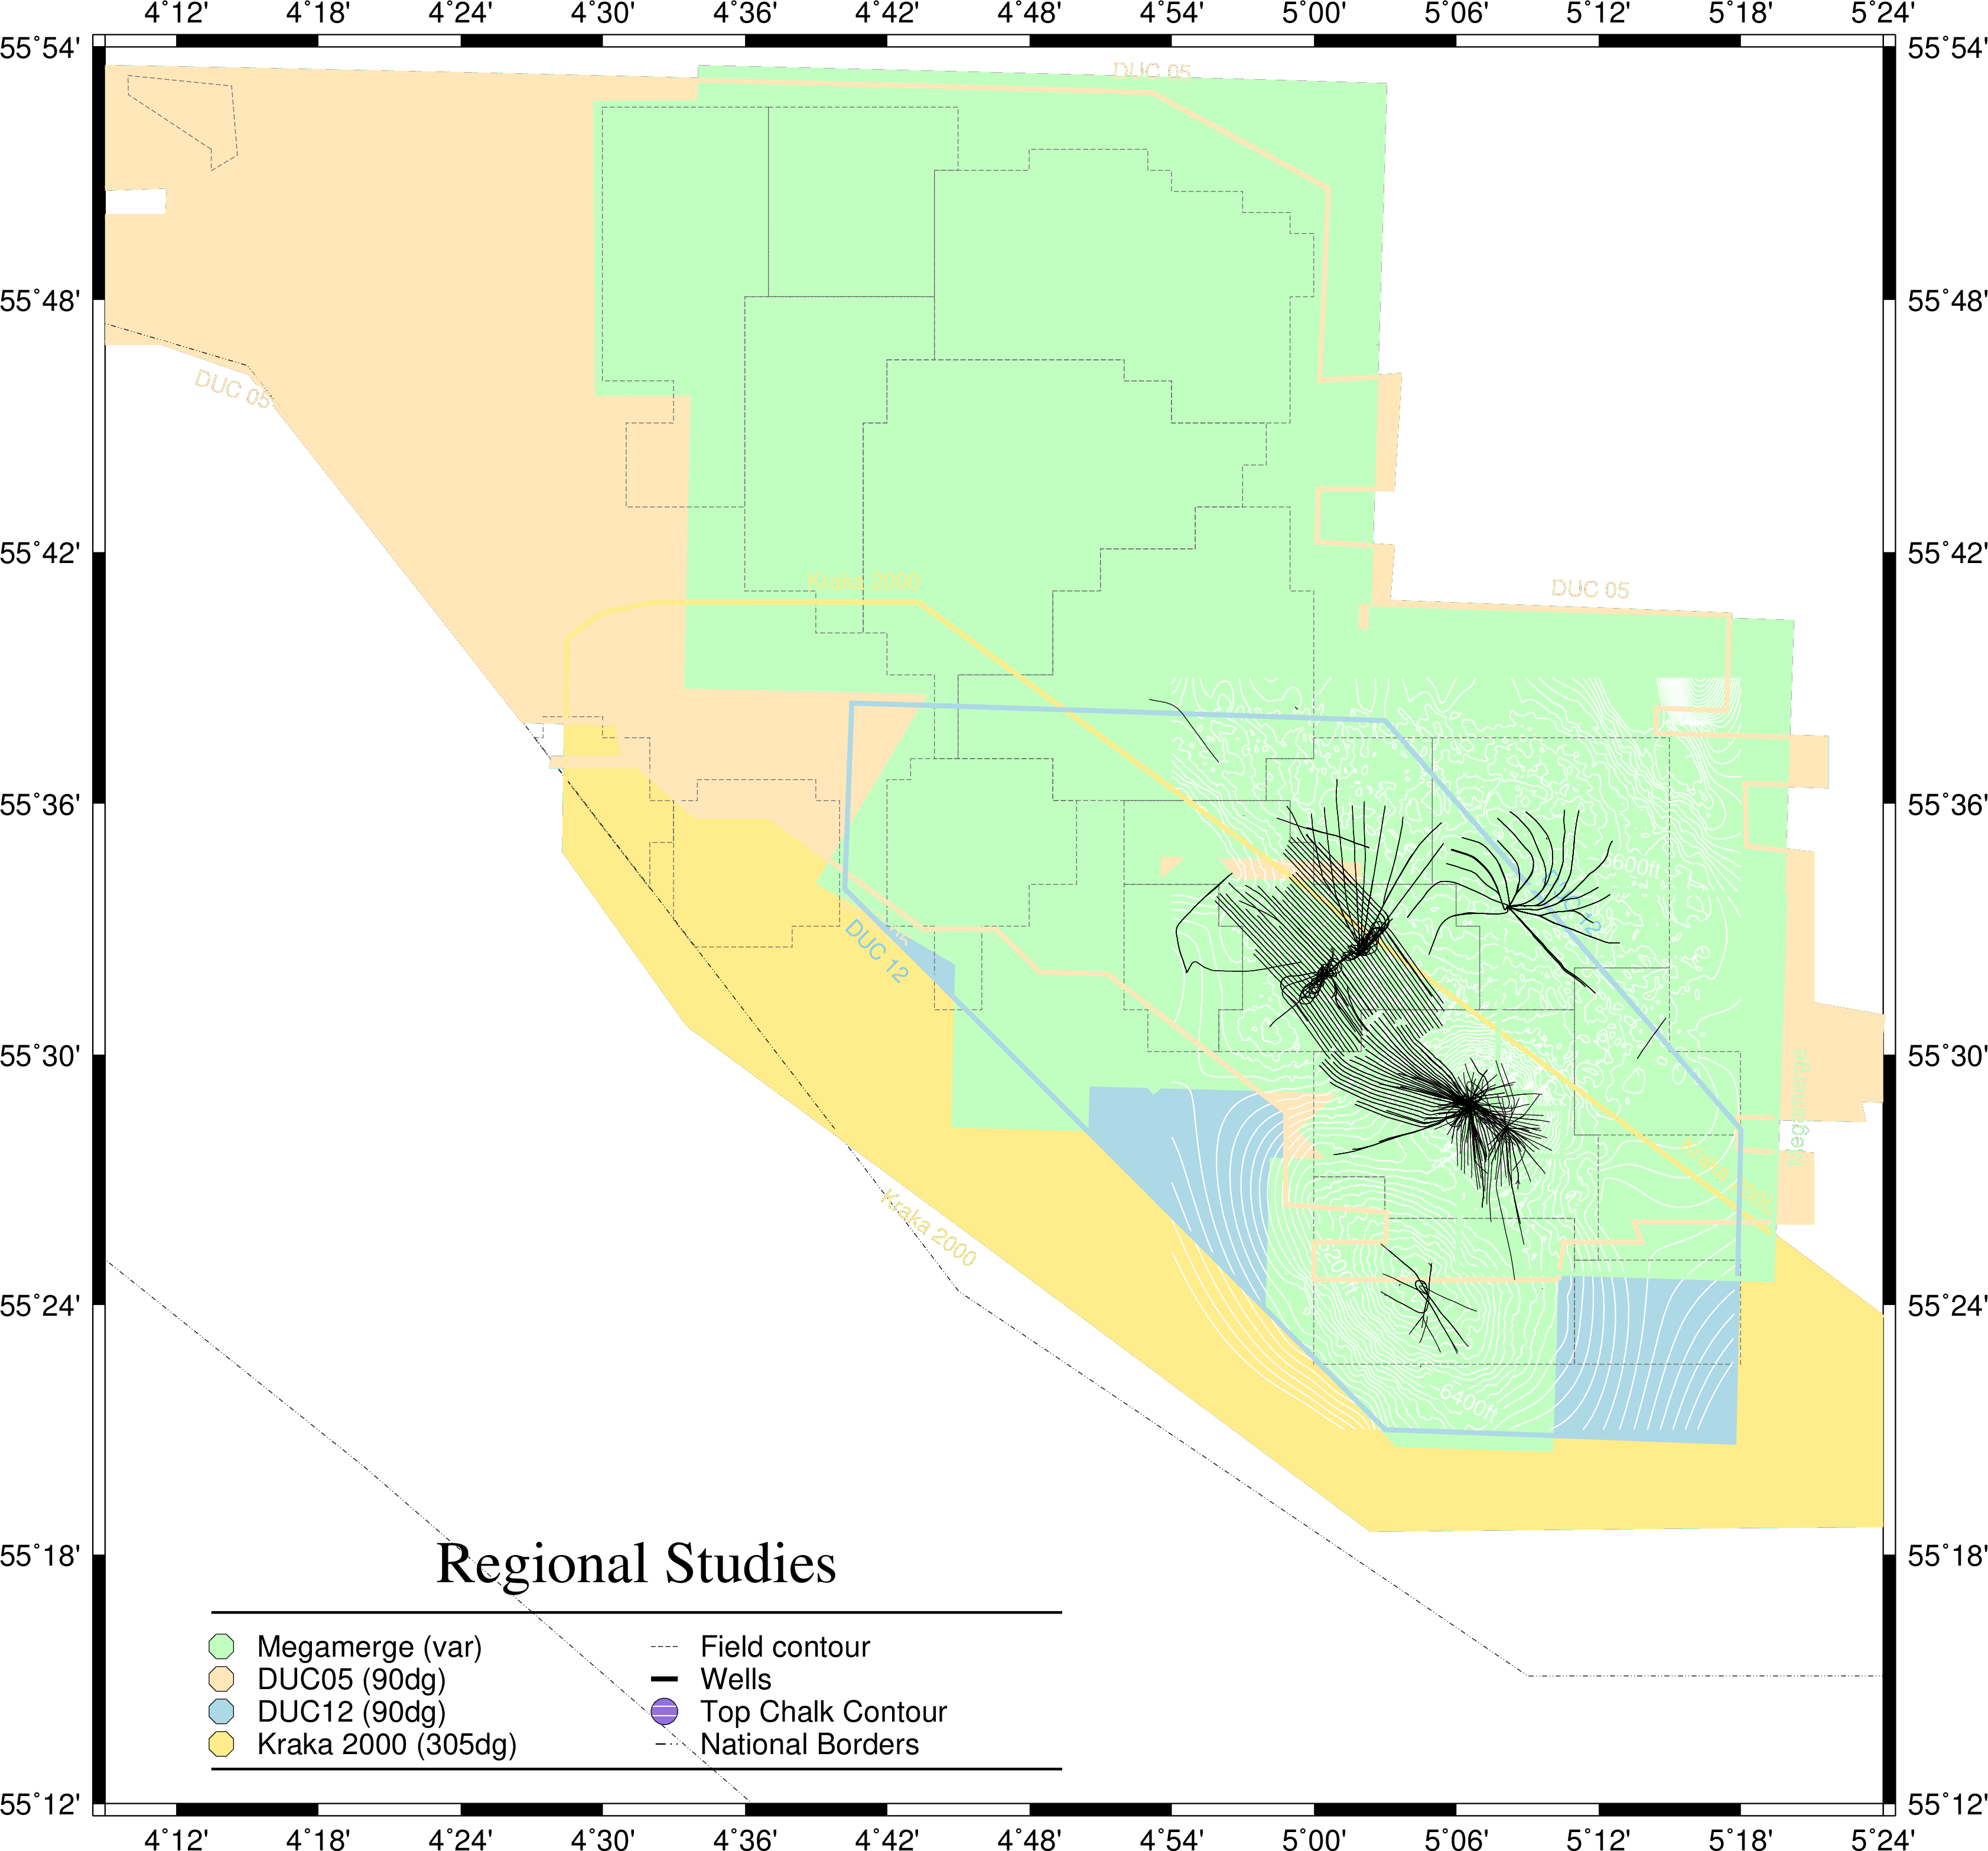
\includegraphics[width=\textwidth]{figures/data/regional.png}
\caption{Regional seismic surveys in the Danish North Sea}
\end{figure}

The regional DUC05 survey covers the entirety of the fields north of Kraka and half of Kraka and Regnar. These surveys were matched in EW (90$^o$) direction \citep{Calvert2014}. The source configuration was kept at a two-source flip-flop configuration at a depth of 5m. The receiver array consists of eight streamers at 100m separation with a near offset at 287m and a length of 6km \citep{Svay2013}, towed at a depth of 7m. The recording system has vastly improved from the 90s surveys (refer to appendix table \ref{kraka-label}). The low filter changed from 8Hz, 6dB/oct to 3Hz, 18dB/oct \citep{Calvert2014}.

The DUC12 survey was extended to cover the entire Kraka field. The streamer configuration was changed to a near-offset of 102m and a length of 4040m \citep{Svay2013}, keeping other parameters constant. The recording system was yet again improved to 2Hz, 6dB/oct as low filter \citep{Calvert2014}. \citet{Dorn-Lopez2005} reference 37 core plugs and according data from the core as well as an elastic reservoir model that relates seismic velocities, porosity, fluid saturation and temperature and \citet{Micksch2014} reference 15 seismic inversion projects on regional data.

\section{Kraka Field Studies}

Kraka is the southernmost field in the Danish North Sea sector. It is part of the salt dome province and forms an anticline structural trap. The regional DUC-05 study covered 50\% of Kraka. The regional DUC12 survey, as well as, the planned DUC16 survey include the whole field \citep{Klinkby2005,GEUSdata}. The Kraka structure was covered by two local studies by Maersk and the \ac{duc} in 1990 and 2000. The Kraka90 survey matches the $90^o$ azimuth of the regional studies and is also included in the Cont-Area  \citep{Jakobsen2010}. The Kraka00 survey, however, was acquired in SE/NW ($305^o$) direction \citep{GEUSdata}. A mismatch of azimuth this large makes the survey virtually ineligible for 4D processing.

A Fugro multiclient survey was acquired across the Danish, Dutch and German North Sea sectors in 2002. The license includes the Kraka field  \citep{Jakobsen2010}. The survey name is Entenschnabel02 (ES02) it was acquired in $90^o$ direction and the acquisition parameters closely matches the \ac{duc} regional surveys as well as the Kraka90 survey \citep{GEUSdata}. The Kraka00 data set is not ideal for 4D purposes. It was used by \citet{Dorn-Lopez2005} to gather valuable information of the reservoir. Hence, a 4D data set exists. Additionally, DUC05 can be used to the extent it covers the field and DUC12 is fully available as 4D monitor. The ES02 data set is suitable for a 4D study, based on the acquisition parameters.

% \begin{figure}[!hbt]
% \centering
% 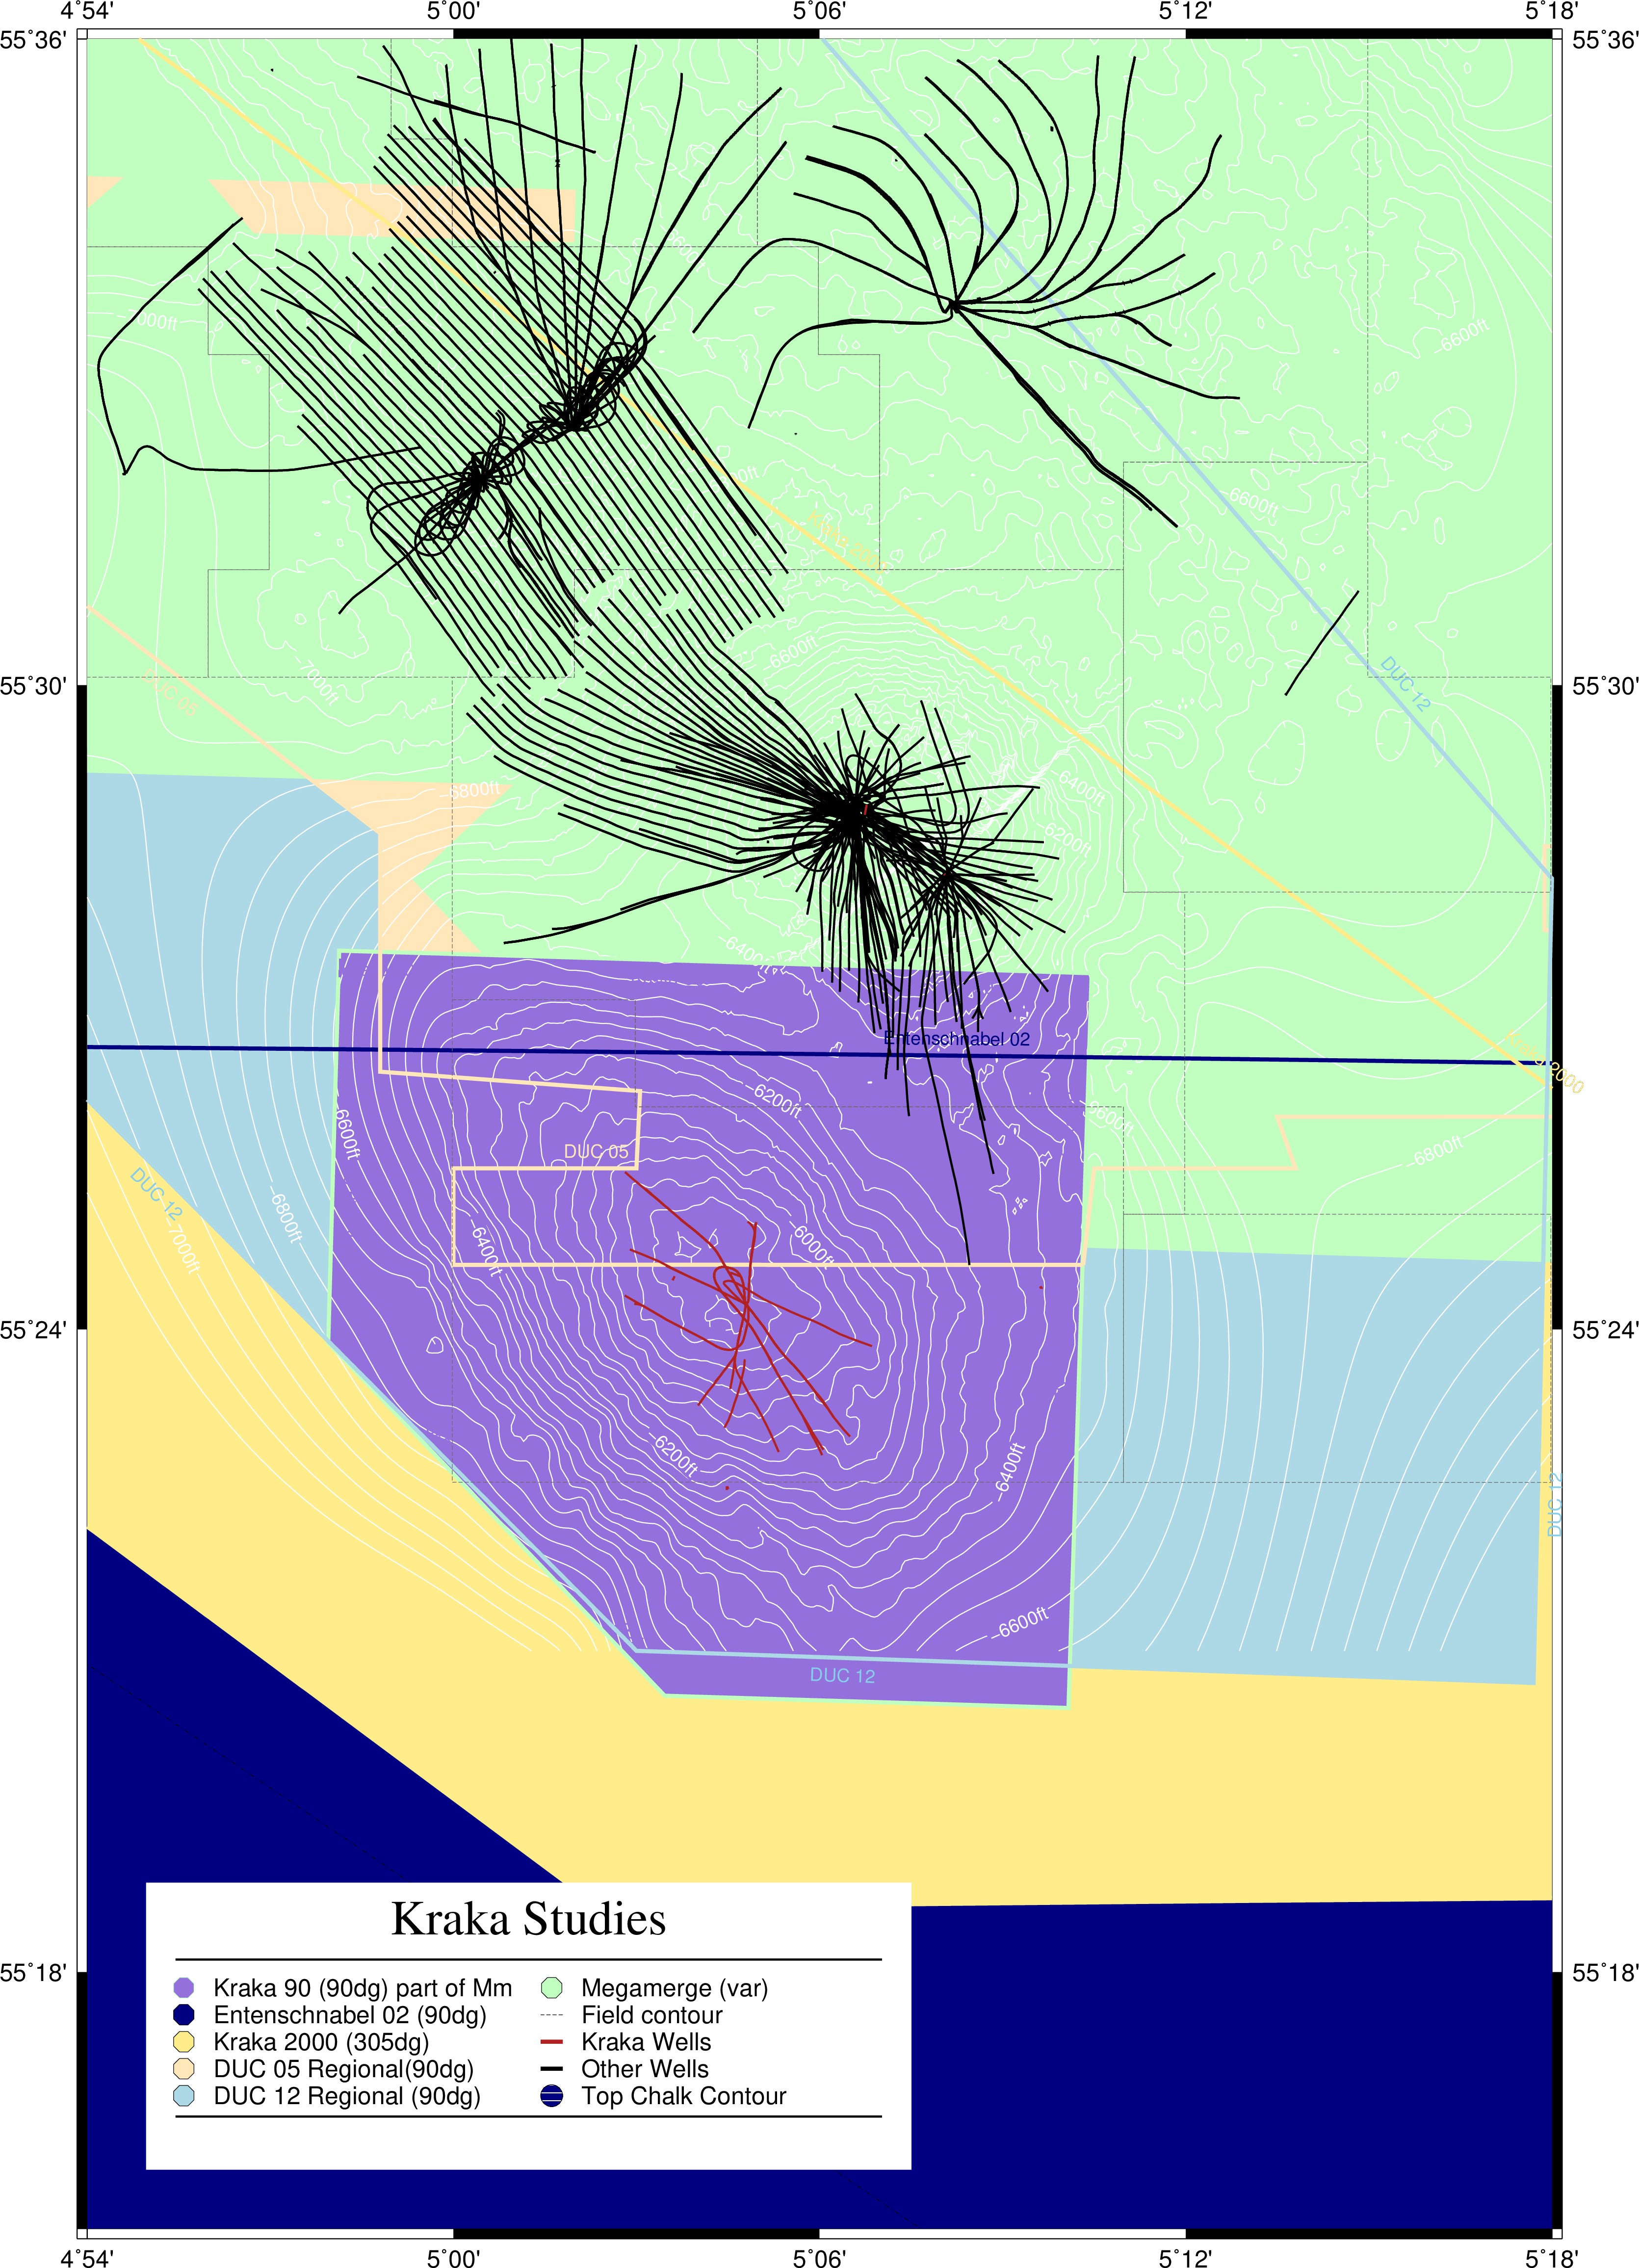
\includegraphics[width=\linewidth]{figures/data/kraka.png}
% \caption{Kraka seismic surveys.}
% \end{figure}

\section{Dan Field Studies}
The Dan field is an anticline structural trap in the salt dome province north of the Kraka structure. It was covered by a local survey in 1988, which is part of the regional Megamerge \citep{Klinkby2005}. The field is fully covered by the two regional surveys DUC05 and DUC12 \citep{Micksch2014, Zaske2014}. These regional surveys with an azimuth of $90^o$ do not match the azimuth of $225^o$ the DAN-88 baseline \citep{Zaske2014}. For this reason a fourth local 3D seismic DAN-05 was acquired in 2005 to match the acquisition geometry for 4D analysis \citep{Zaske2014}.

The Kraka00 survey covers the Dan field. It was intended as a 4D monitor but differing acquisition geometries and parameters make the processing a very difficult task \citep{Dorn-Lopez2005}. Additionally, a ocean bottom node (OBN) 3D survey DAN-12 was acquired in 2012. This survey was matched to the DUC-12 streamer data. The grid spacing was 225mx225m with 959 nodes and 37.5m shot distance \citep{Zaske2014}. In total two baseline surveys and two matching monitors are available, making up a total of two 4D data sets \citep{Zaske2014} and four inversion projects \citep{Micksch2014}.

% \begin{figure}[hbtp]
% \centering
% 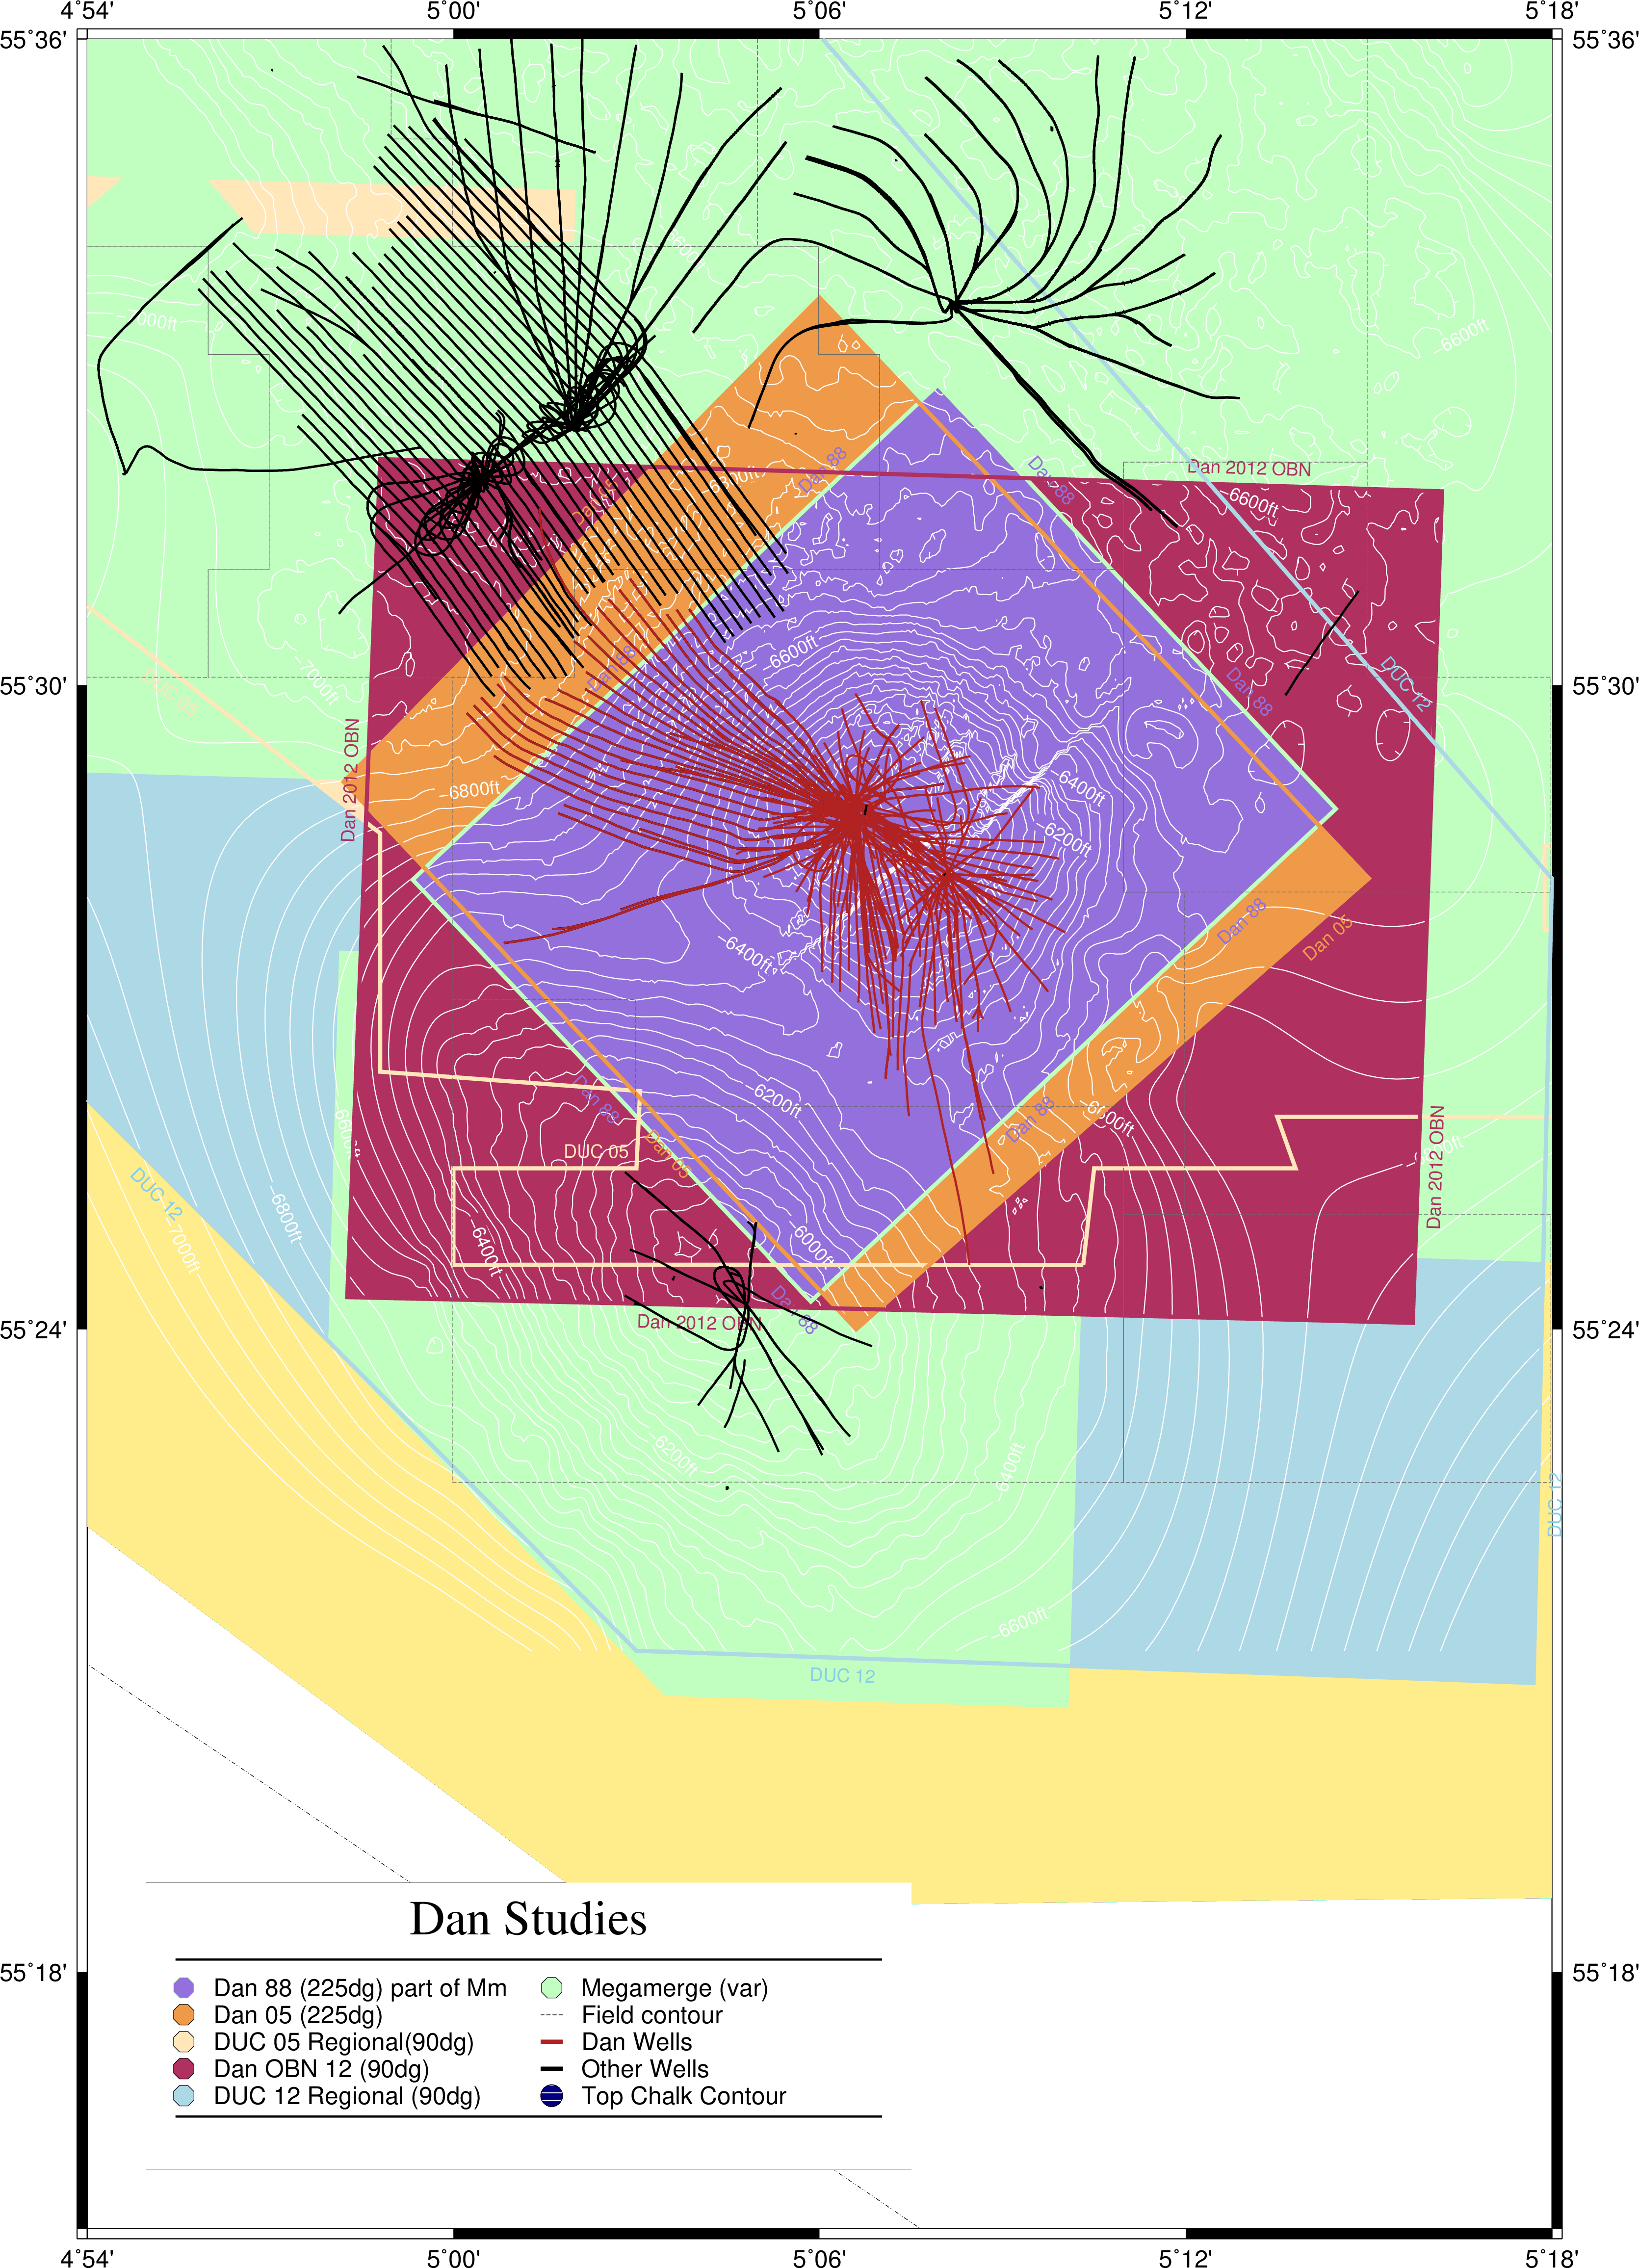
\includegraphics[width=\linewidth]{figures/data/dan.png}
% \caption{Dan seismic surveys.}
% \end{figure}

\section{Halfdan Field Studies}

The Halfdan area is a non-structurally trapped reservoir NW of the Dan structure. The baseline survey is the SKJOLD-92 survey in EW (90\textsuperscript{o}) direction \citep{Calvert2014}. This survey is also part of the regional contiguous migration area \citep{Klinkby2005}. The DUC05 and DUC12 regional monitor surveys match the EW (90\textsuperscript{o}) direction of the baseline \citep{Calvert2014}.

Two 4D studies are available \citep{Calvert2014} in addition to 4D simulations for the 2012 - 2005 study \citep{Calvert2013,Calvert2014}.

\begin{figure}[!hbp]
    \centering
    \subbottom[Kraka Field Seismic Data]{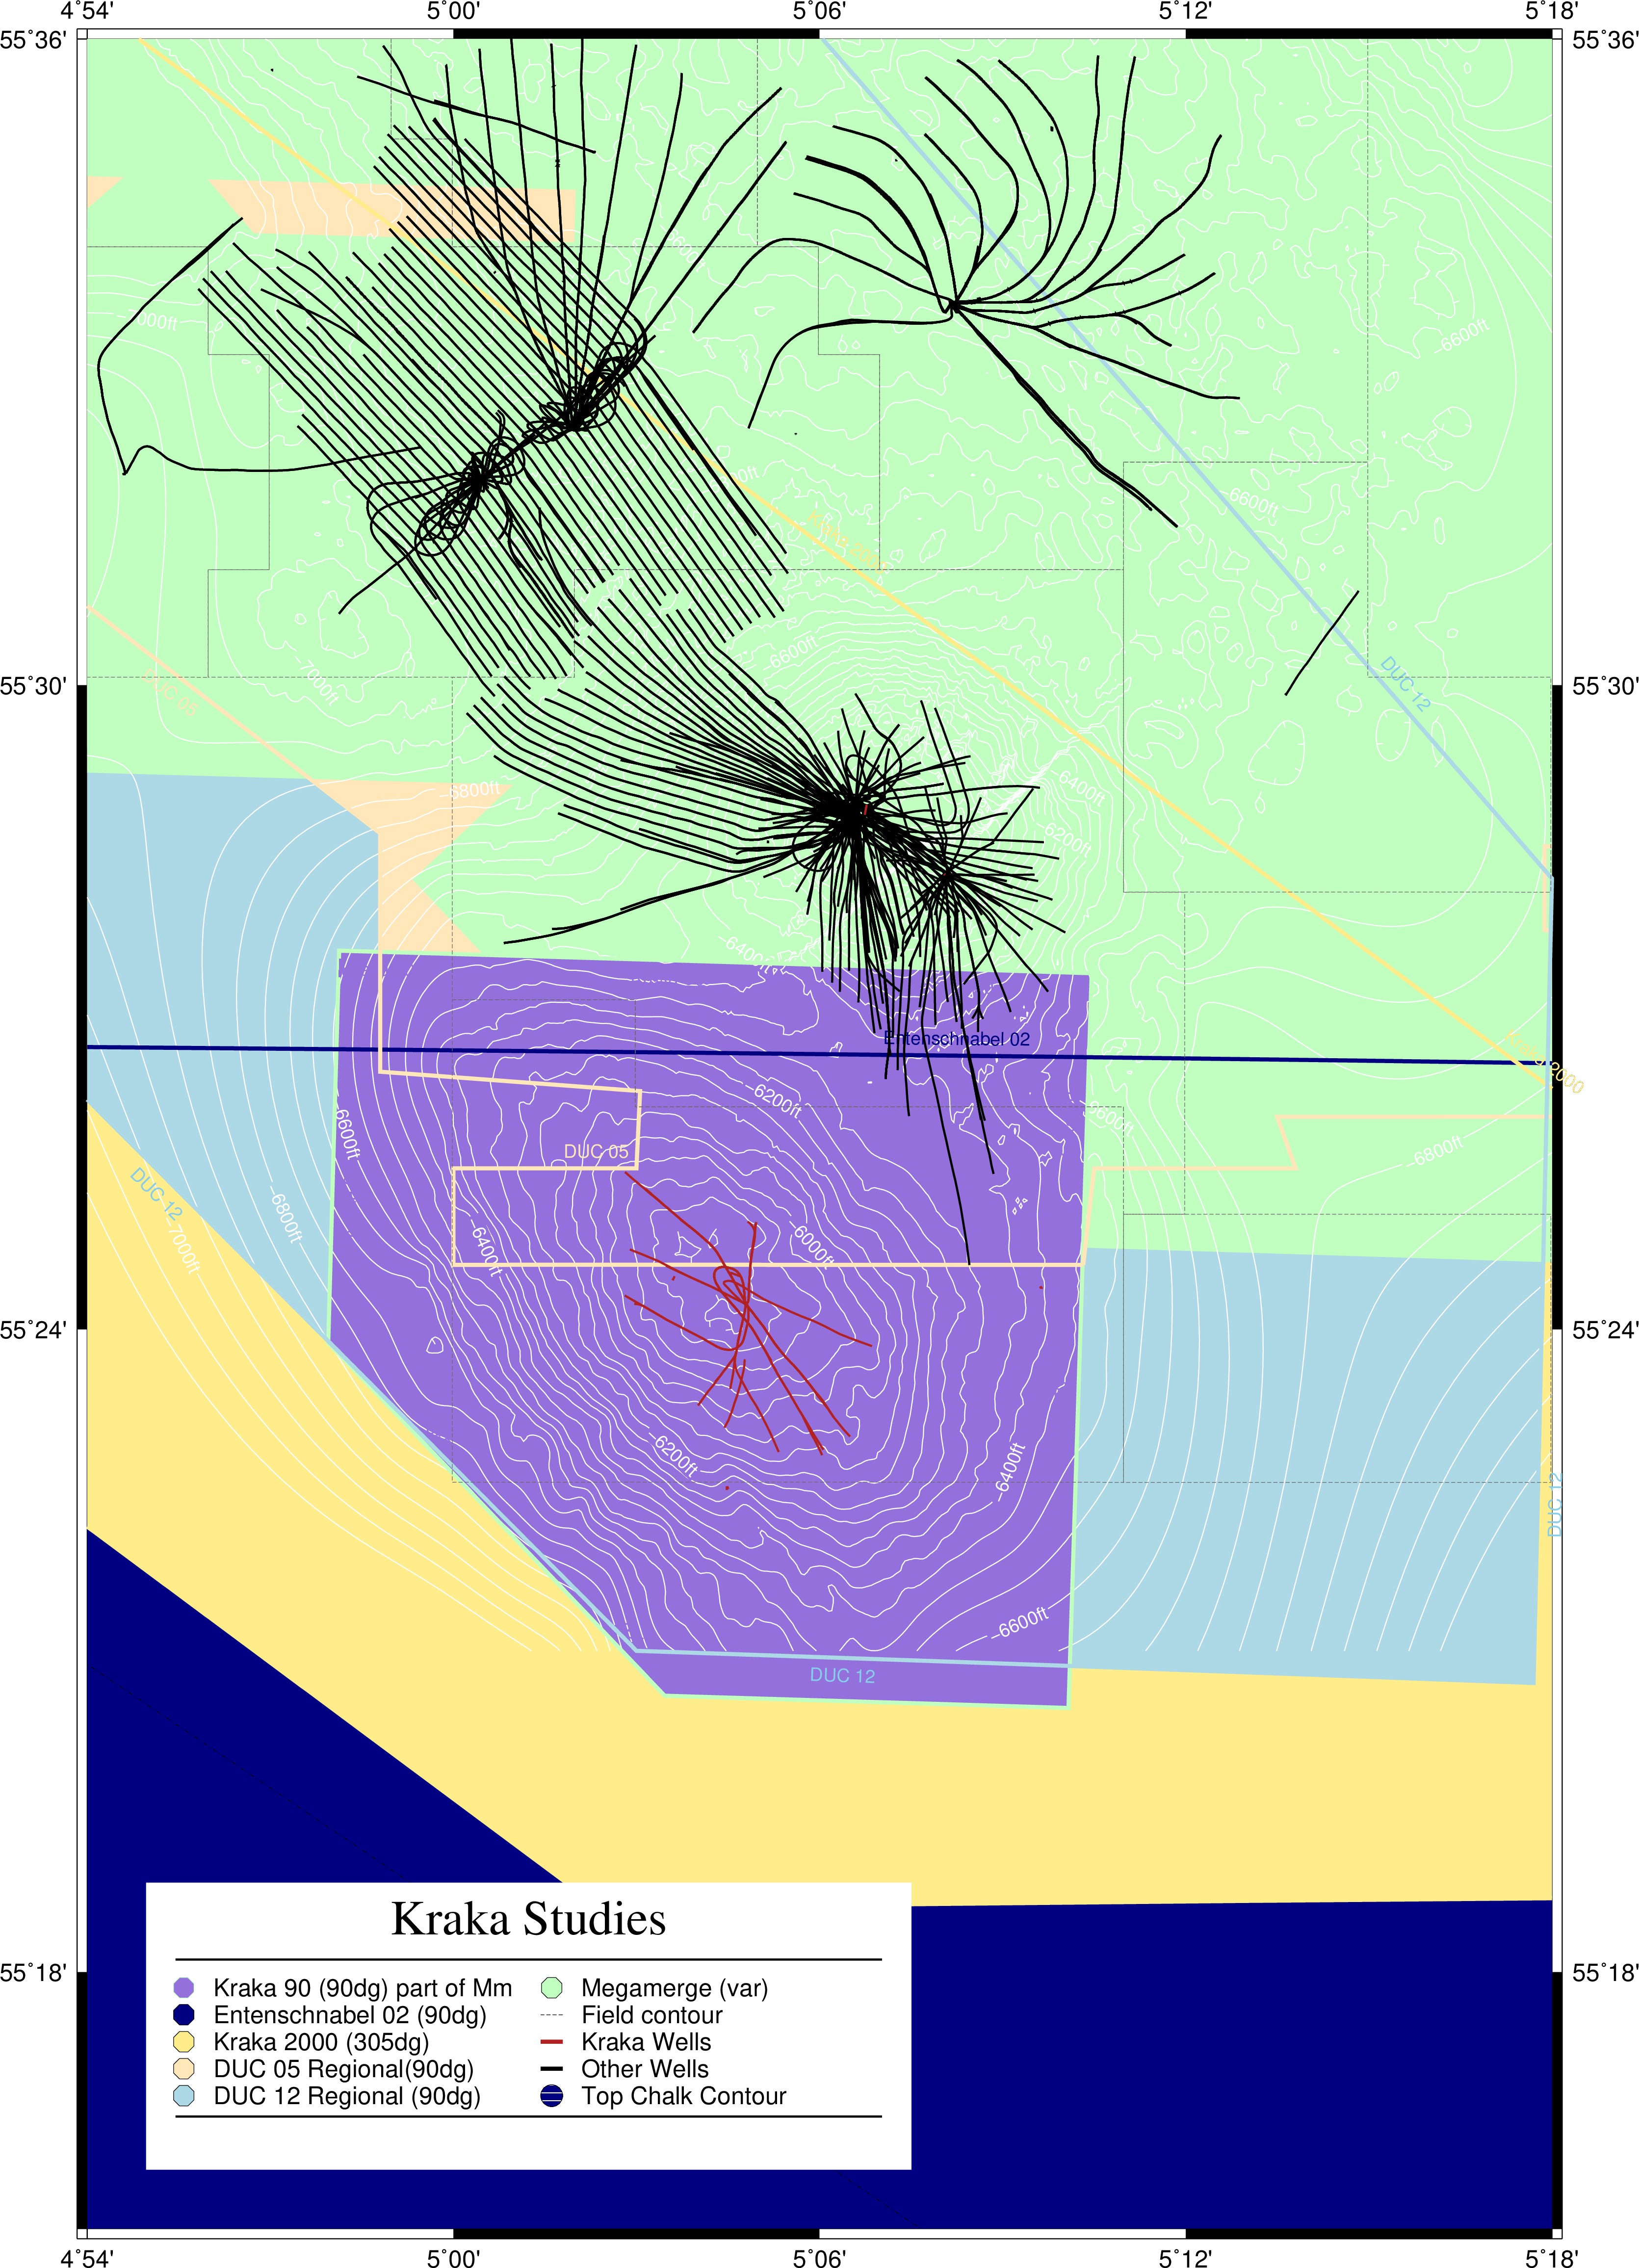
\includegraphics[width=.35\textwidth]{figures/data/kraka.png}\label{fig:kraka}}%
    \subbottom[Dan Field Seismic Data]{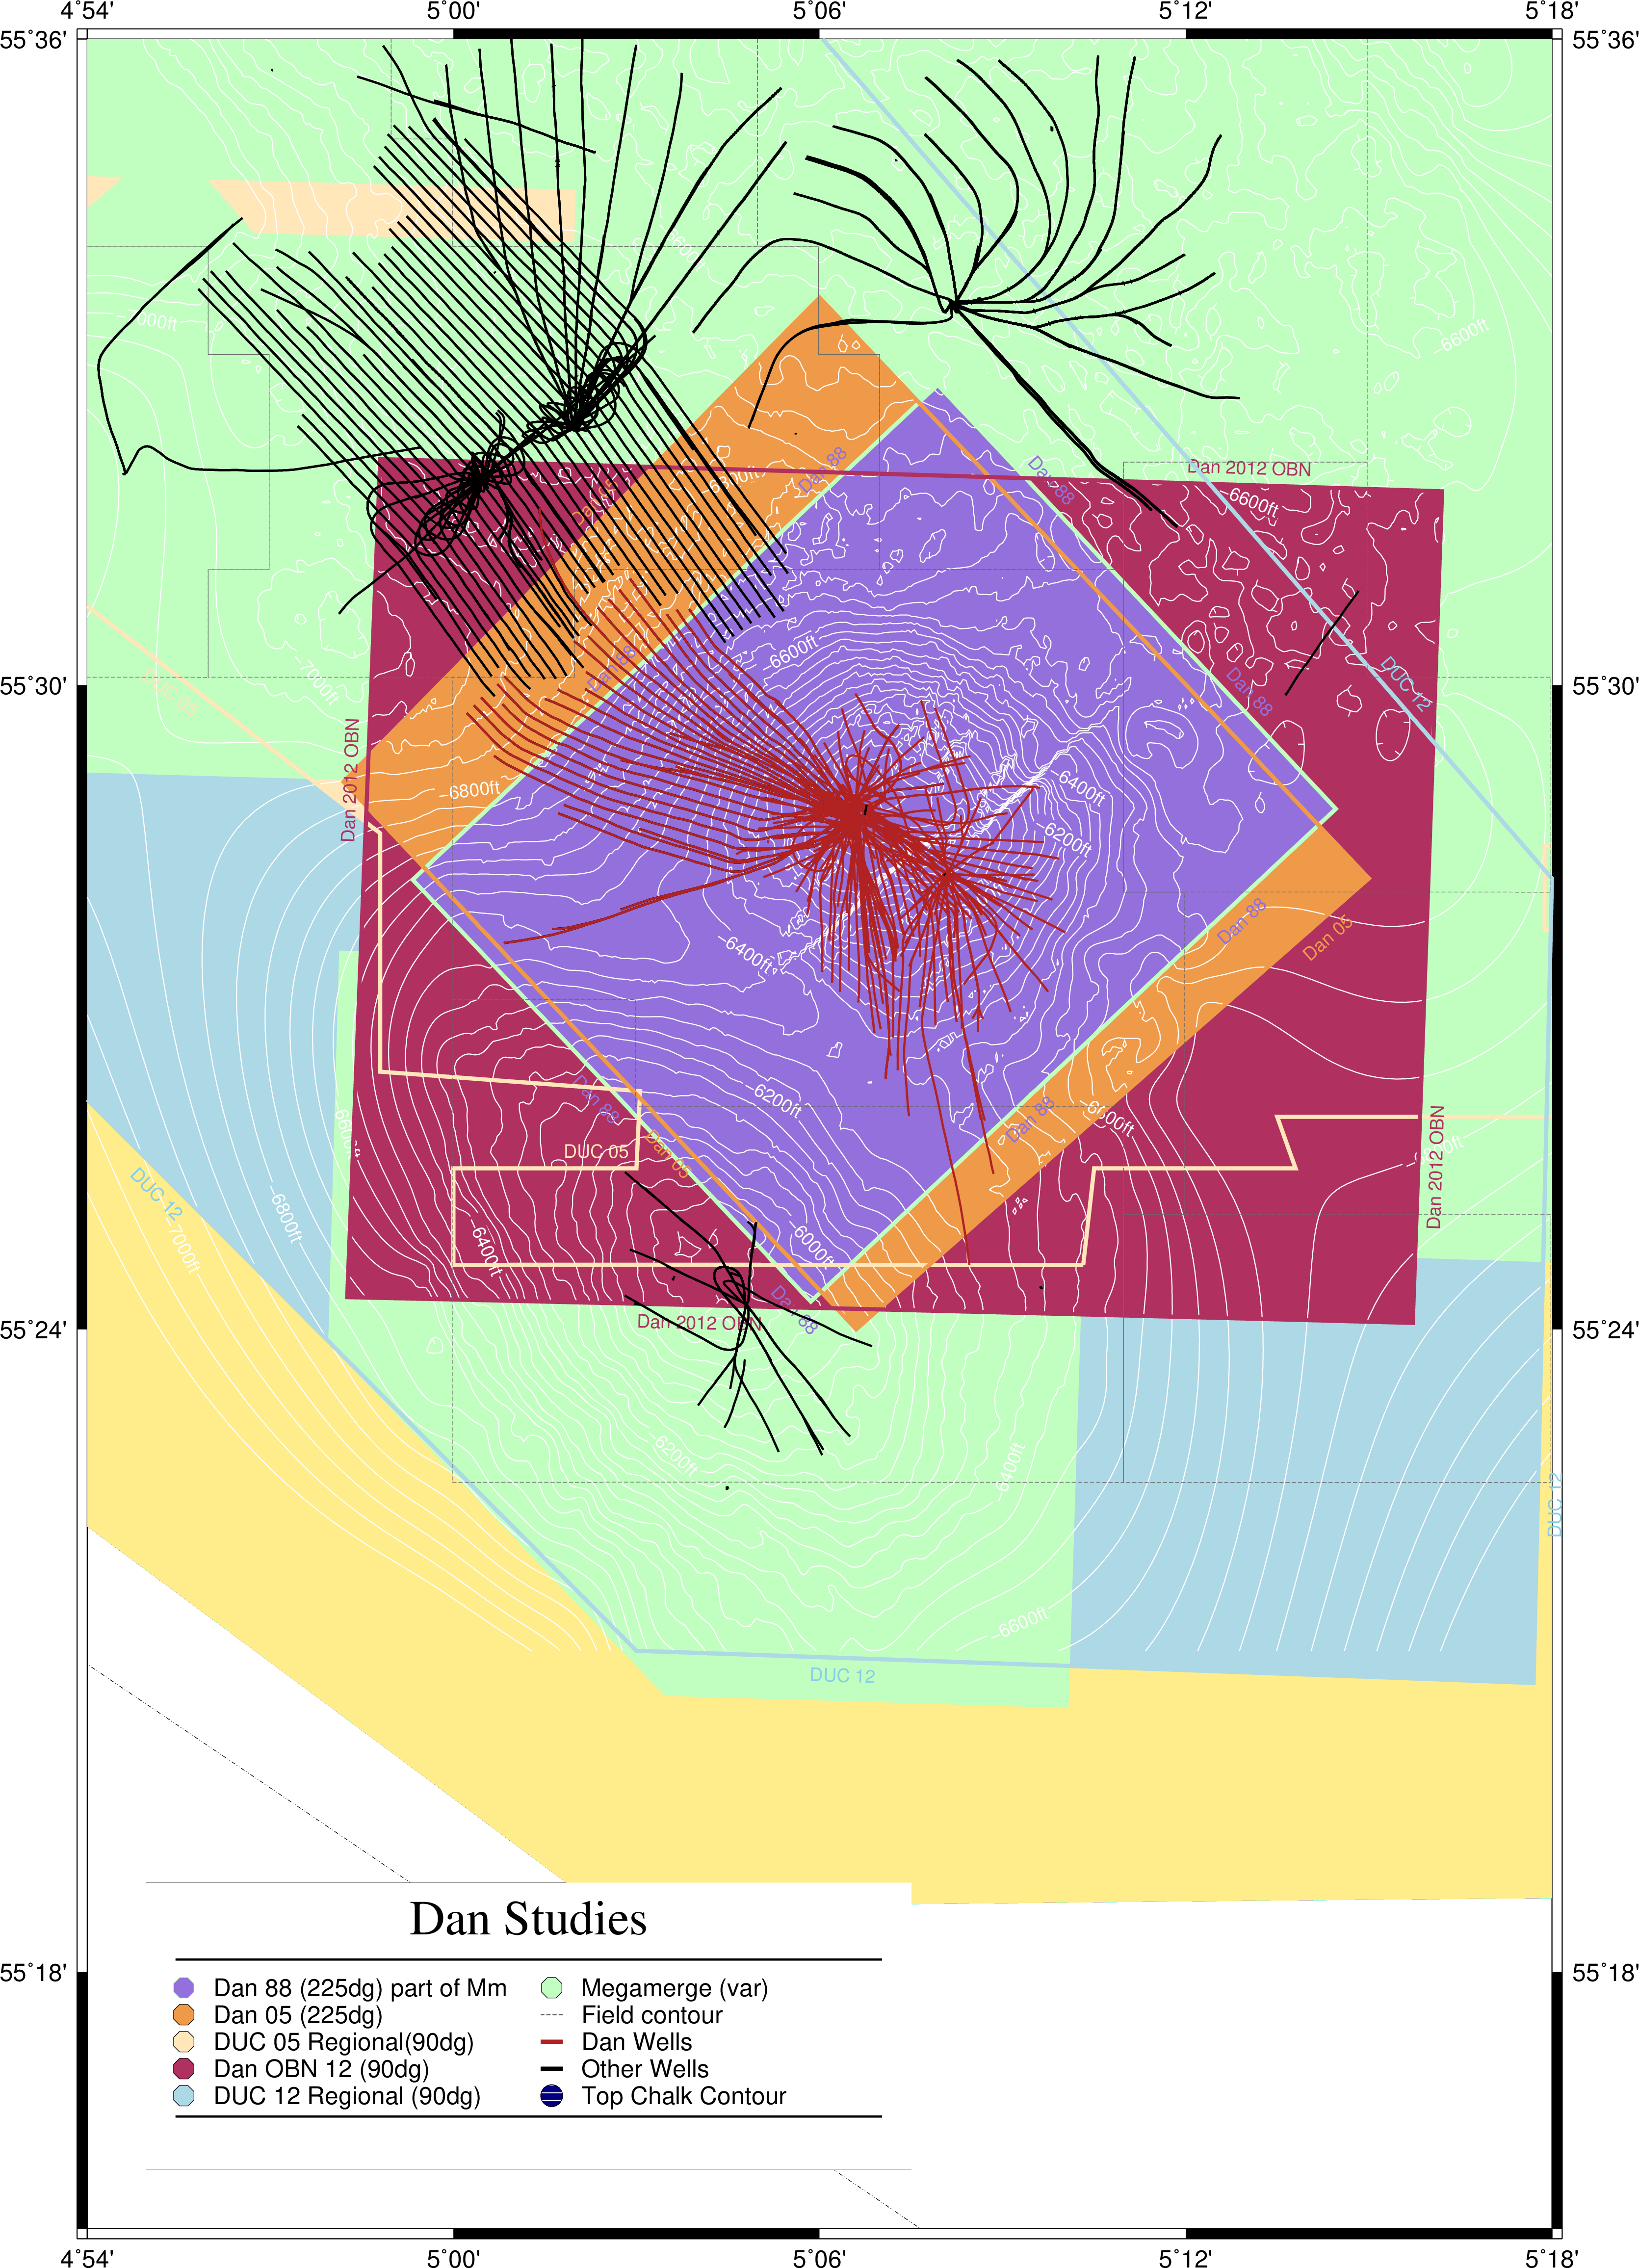
\includegraphics[width=.35\textwidth]{figures/data/dan.png}\label{fig:dan}}%
    \subbottom[Halfdan Field Seismic Data]{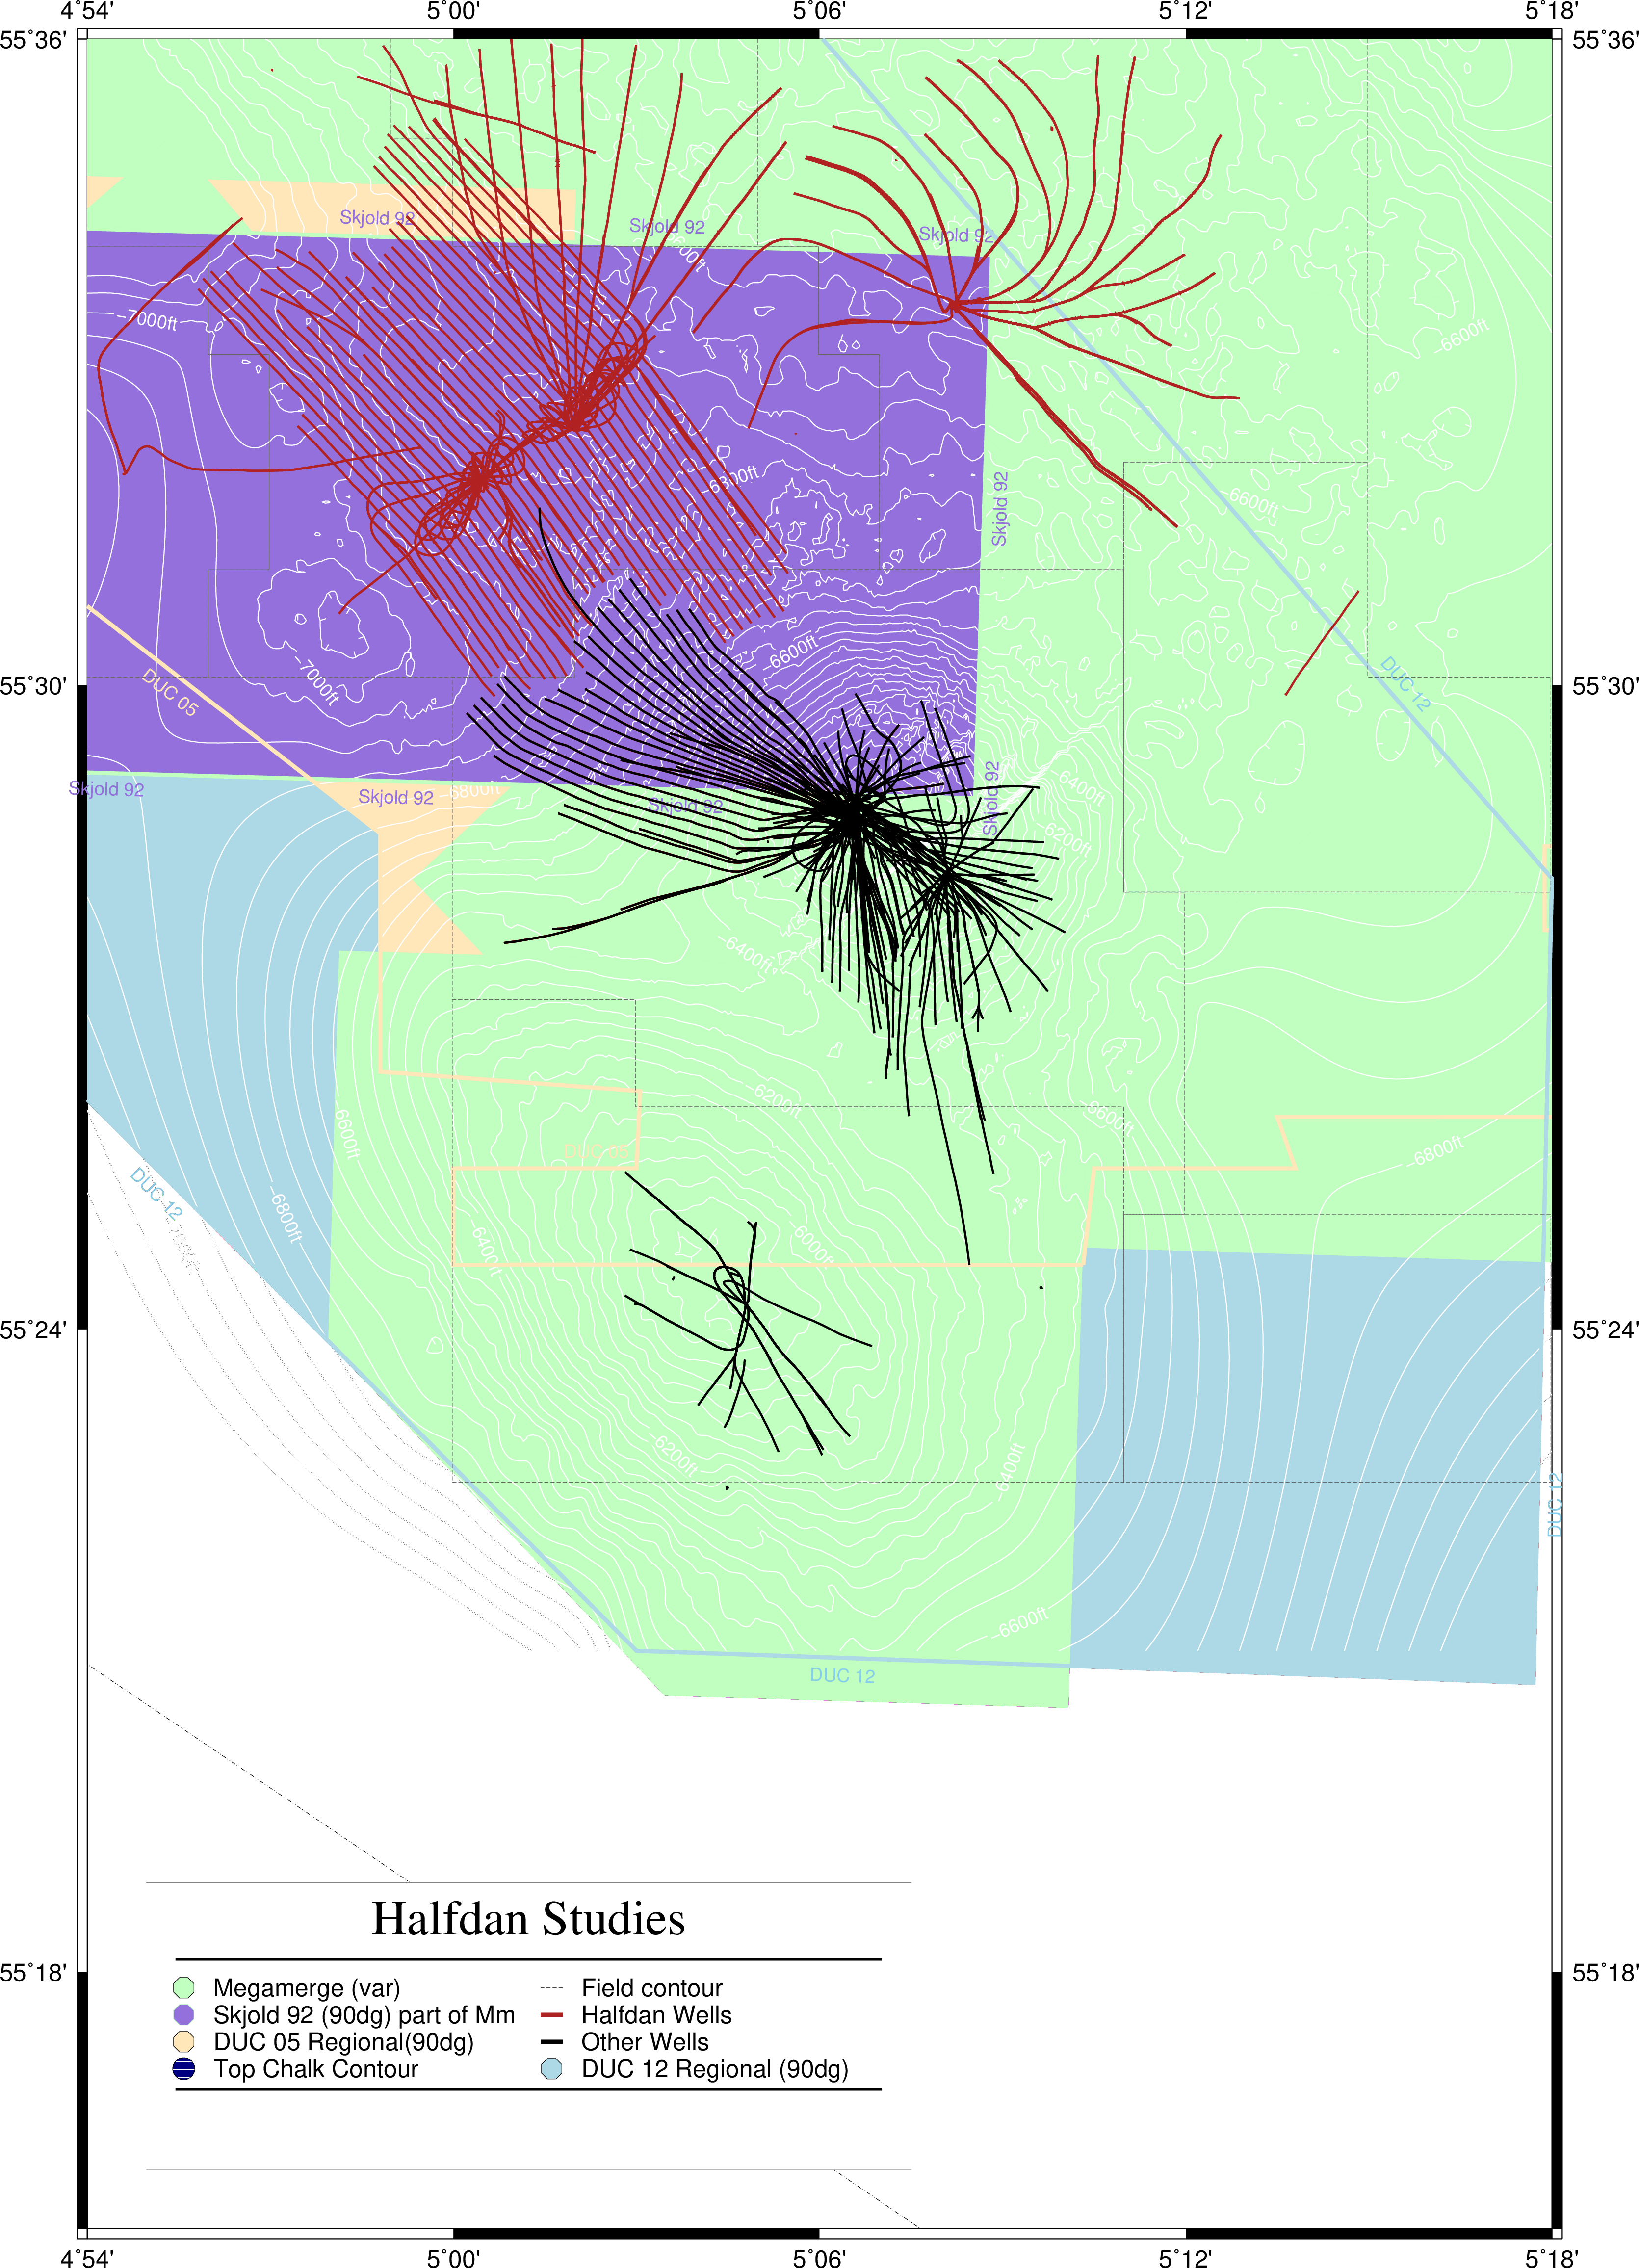
\includegraphics[width=.35\textwidth]{figures/data/halfdan.png}\label{fig:halfdan}}%
    \caption{Seismic surveys in the Danish North Sea extraced from \citet{GEUSdata}. Large versions and additional information on surveys in \cref{app:data}}
    \label{fig:seismic-surveys}
\end{figure}